\documentclass{article}
\usepackage[a4paper, total={7in, 9in}]{geometry}
\usepackage[version=3]{mhchem} % Package for chemical equation typesetting
\usepackage{siunitx} % Provides the \SI{}{} and \si{} command for typesetting SI units
\usepackage{graphicx} % Required for the inclusion of images
%\usepackage{natbib} % Required to change bibliography style to APA
\usepackage{amsmath} % Required for some math elements
\usepackage{booktabs}
\usepackage{physics}
\usepackage{minted}
\usepackage{subcaption}
\usepackage[english]{babel}
% Use the palatino font
\usepackage[sc]{mathpazo}
\usepackage[backend=biber,
    style=numeric,
    bibencoding=utf8,
    maxcitenames=2,
]{biblatex}
\addbibresource{bibliography.bib}

\usepackage{hyperref}
\hypersetup{%
	pdfpagelabels=true,%
	plainpages=false,%
	pdfauthor={Angus Hollands},%
	pdftitle={Year 4 MEng. Practical Monte Carlo using MCNP },%
	% pdfsubject={Determining the Velocity of Photons},% TODO
	bookmarksnumbered=true,%
	colorlinks=false,%
	citecolor=black,%
	filecolor=black,%
	linkcolor=black,% you should probably change this to black before printing
	urlcolor=black,%
	pdfstartview=FitH%
}



\setlength\parindent{0pt} % Removes all indentation from paragraphs
\DeclareSIUnit\neutron{n}

  % \renewcommand{\labelenumi}{\alph{enumi}.} % Make numbering in the enumerate environment by letter rather than number (e.g. section 6)

%\usepackage{times} % Uncomment to use the Times New Roman font

\title{Practical Monte Carlo using MCNP \\ Assessed exercises} % Title

\author{Angus \textsc{Hollands}} % Author name

\date{\today} % Date for the report

\begin{document}

\maketitle % Insert the title, author and date


\begin{abstract}
  A Monte Carlo simulation was performed for \num{20000} source histories, to model the light water moderated neutron fluence from a fission neutron source through the sides of a stainless steel bucket. The resulting fluence histograms were recorded, plotted against energy, and the statistical reliability of the data evaluated. One set of tally results were not found to be reliable after failing the tally fluctuation chart (TFC) Figure of Merit (FoM) slope test. The simulation was subsequently repeated for \num{200000} source histories, and the corresponding statistical reliability of the data re\textendash evaluated. It was found that simulating \num{200000} source histories was sufficient for both flux tallies to pass the ten TFC tests, indicating result reliability.
  A second Monte Carlo model was designed to investigate the effective multiplication factor $k_{\text{eff}}$ of a simplified four cylinder enriched uranium reactor system. Several simulations were performed for two moderators (graphite, light water) and two enrichments (\SI{20}{\percent}\ce{^{235}U}, \SI{25}{\percent}\ce{^{235}U}). The values for $k_{\text{eff}}$ were found (in product order) to be \num{0.79340 \pm 0.00075}, \num{0.93439 \pm 0.00075}, \num{0.84532 \pm 0.00076}, and \num{1.00507 \pm 0.00078}, respectively.
\end{abstract}

\section{Introduction}
The Boltzmann neutron transport equation (see Eq~\ref{eq:transport}, for the integral form describing a non multiplying medium with a time\textendash independent source) is a description of the macroscopic processes governing the conservation of neutrons within a system.
\begin{equation}
  \label{eq:transport}
  \left(\vb{\Omega}\dotproduct\vb{\nabla}+\Sigma_t(\vb{r},E)\right)\phi(\vb{r},E,\vb{\Omega})=\int_{4\pi}{\int_0^\infty{\Sigma_s(\vb{r},E^\prime\rightarrow E,\vb{\Omega^\prime}\rightarrow\vb{\Omega})\phi(\vb{r},E^\prime,\vb{\Omega^\prime})\dd{E^\prime}}\dd{\vb{\Omega^\prime}}}+s(\vb{r},E,\vb{\Omega})
\end{equation}
Though simple to derive from conventional transport theory, analytical solutions are difficult for simple systems, and effectively impossible for those which are complex. Instead, one must solve the transport equation numerically, either by deterministic or stochastic methods. In the former case, one can discretise the problem along each of its dimensions, and solve a set of matrix equations which describe the behaviour of the (local) system. Though quick to find an approximate solution, its performance is heavily dependent upon the simplicity of the problem, with complex geometries and complicated neutron spectra demanding an explicit compromise between model accuracy and performance. Stochastic methods (or Monte Carlo methods) instead simulate the relevant physical processes themselves, where the parameters of the processes are sampled from known probability distributions. As more and more of the problem space is sampled, the MC solution approaches the "true" solution (distribution). Though computationally expensive, by means of convergence, these methods may be more accurate than the deterministic approach.

As well as the fission\textendash free transport equation, the Monte Carlo approach can also be used to solve the k\textendash eigenvalue transport equation of the form
\begin{equation}
  \label{eq:k_eigenvalue_transport}
  \left(\vb{\Omega}\dotproduct\vb{\nabla}+\Sigma_t(\vb{r},E)\right)\phi(\vb{r},E,\vb{\Omega})=\int_{4\pi}{\int_0^\infty{\Sigma_s(\vb{r},E^\prime\rightarrow E,\vb{\Omega^\prime}\rightarrow\vb{\Omega})\phi(\vb{r},E^\prime,\vb{\Omega^\prime})\dd{E^\prime}}\dd{\vb{\Omega^\prime}}}+\frac{1}{k}\frac{\chi(E)}{4\pi}s(\vb{r},E,\vb{\Omega})
\end{equation}
for $k$, where $\chi(E)$ describes the emission spectrum of the fission neutrons. The largest eigenvalue $k$ quantifies the effective level of neutron multiplication $k_{\text{eff}}$ within the system. The state of the system is then given by Table~\ref{table:k}
\begin{table}[]
\centering
\caption{My caption}
\label{table:k}
\begin{tabular}{@{}ll@{}}
\toprule
Condition & State          \\ \midrule
$k < 1$   & Sub-critical   \\
$k = 1$   & Critical       \\
$k > 1$   & Super-critical \\ \bottomrule
\end{tabular}
\end{table}
% system is critical if TINN sol to source free trans eq can be found

In this report, the Monte Carlo N-Particle (MCNP) code is used to determine the neutron flux along the external walls of a model reactor vessel. The model geometry is defined using the various non\textendash macrobody primitives available, and the surface tallying feature used to obtain two energy dependent histograms describing the neutron fluence distribution incident upon the problem surfaces. An investigation is performed into the conditions under which these tally data are invalidated. To provide a neutron source for this model, the Watt Fission prompt neutron spectrum for \ce{^{235}U} is used, with parameters referenced from the MCNP user manual.

Subsequently, the MCNP KCODE k\textendash eigenvalue transport equation solver is used to investigate the effect of varying parameters such as the moderator material and fuel enrichment upon the reactor criticality.

\section{Method}
  \subsection{Exercise 1}
    \label{sec:ex_1}
    An MCNP input file was written to design the simulation model (see Appendix~\ref{lst:ex_1}). A stainless steel vessel (of  density \SI{7.92}{\gram\per\cm^3}) with internal base \SI{10}{\cm} by \SI{20}{\cm}, wall thickness \SI{2}{\mm}, and external height \SI{20}{\cm} was modelled as the intersection between two cuboids, centered about the z axis with the lower floor placed at $z=0$.
    \begin{figure}[htb]
      \centering
      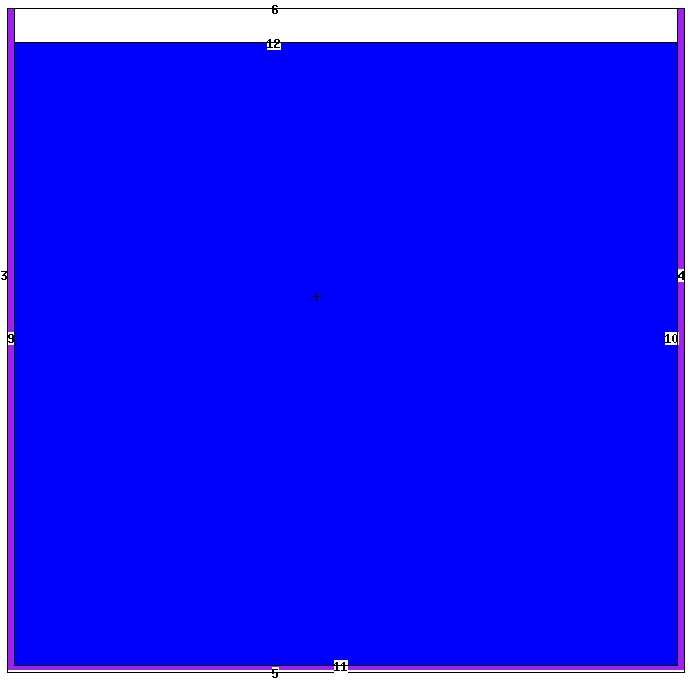
\includegraphics[width=0.3\textwidth]{cuboid.png}
      \caption{2D XZ plot of Exercise 1 geometry.}
      \label{fig:ex_1_geometry}
    \end{figure}
    The moderator was defined as the intersection between the internal cuboid and an infinite planar surface of normal $\mqty(0 & 0 & -1)$ at $\mqty(0 & 0 & 19.0)$. Two void regions were then defined, one for the volume outside of the outer cuboid, and the other for the region between the moderator surface and the plane bounding the outer cuboid ceiling.

    All cells were defined with a neutron importance of $1$, apart from the outer void region, assigned with the correct weight density (apart from the outer void region), and their materials appropriately defined in the DATA section with the appropriate atomic / weight composition. The moderator material was assigned the light water low energy cross section library \textit{lwtr.01[t]}.

    Two surface neutron flux tally cards were defined, using a common set of energy bins, with upper bin edges defined along the log\textendash linear interval between \SI{1e-9}{\MeV} and \SI{10}{\MeV}. One tally recorded the \textit{average} flux through the two short external sides of the vessel, and the other recorded the corresponding flux through the two larger sides.

    A thermal neutron source with an energy distribution given by the Watt Fission spectrum for \ce{^{235}U} (see Fig~\ref{fig:watt_fission}), with parameters $a=0.988$, $b=2.249$, was placed at $\mqty(0 & 0 & 2.2)$, and the simulation performed for \num{20000} neutrons (MODE N) source histories. A secondary simulation was performed with an increased number of source histories of \num{210000}.
    \begin{figure}[htb]
      \centering
      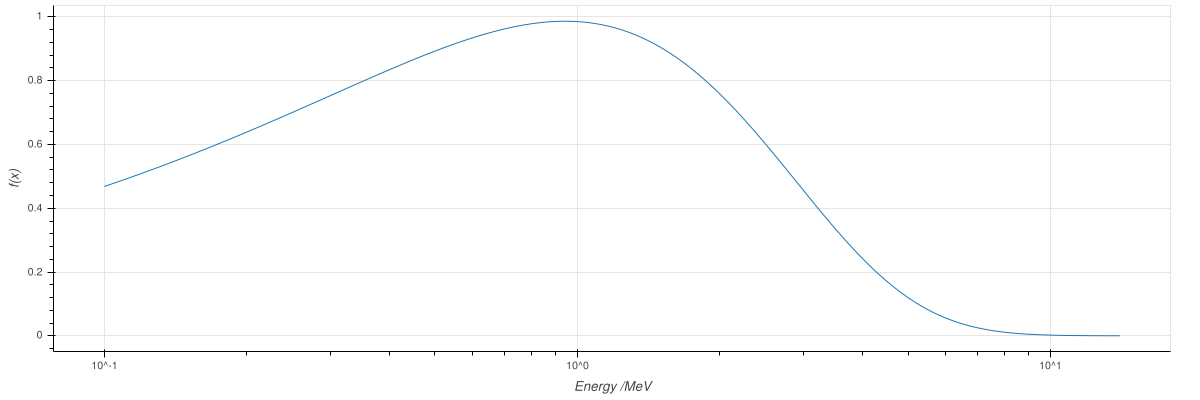
\includegraphics[width=\textwidth]{watt_spectrum_235_u.png}
      \caption{Watt Fission spectrum for prompt neutrons (\ce{^{235}U}).} % TODO chite https://ac.els-cdn.com/S1875389215001236/1-s2.0-S1875389215001236-main.pdf?_tid=946afe26-9e8b-4e65-afa5-899d0c8d8665&acdnat=1523017641_ed02eb00bf5004212d9cca7c0116a978
      \label{fig:watt_fission}
    \end{figure}

  \subsection{Exercise 3}
    The geometry described in Section~\ref{sec:ex_1} was modified such that the internal base measured \SI{100}{\cm} by \SI{100}{\cm}, with an external height of \SI{60}{\cm}.
    A concrete floor was defined, of thickness \SI{150}{\cm}, and a lateral radius of \SI{200}{\cm}. These two parameters were not defined in the exercise requirements. The former was informed by the thickness of a conventional reactor containment vessel\cite{nuclear_reactors} and an approximate \SI{0.025}{\percent} attenuation calculation (see Eq~\ref{eq:attenuation}). From literature, the value of $\Sigma_R$ is approximately $0.04$\cite{neutrons}. The latter was chosen as the radius of the smallest conventional reactor core diameter. % TODO explain why
    \begin{align}
      \label{eq:attenuation}
      I(x)&=I_0\exp(-\mu x) //
      \mu &= \frac{1}{\Sigma_R}//
      x &= -\frac{\ln{\frac{I(x)}{I_0}}}{\mu}
    \end{align}
    The definition of a concrete floor serves an additional purpose to shielding; to reflect a fraction of the neutrons back into the vessel.
    The moderator volume was resized to satisfy the original wall thickness constraints, and the surface moved to \SI{2}{\cm} from the ceiling of the vessel. For each simulation, the appropriate moderator material was defined (for graphite / water), and the corresponding low energy cross section library referenced (\textit{lwtr.01[t]} / \textit{grph.01[t]})

    Four enriched uranium cylindrical sources, of radius \SI{7.5}{\cm} and height \SI{25}{\cm}, were placed within the moderator cell, which served as fissile material for the KCODE algorithm. Their corresponding material card was defined for a by\textendash weight enrichment which was varied across several of the simulations. The primary neutron sites for the solver were provided as initialisation parameters for the algorithm, using the KSRC card, which distributed 1000 starting neutrons across the centroids of the uranium cylinders. The KCODE algorithm was configured for a warm up of 200 cycles, with an initial reactivity estimate of 1.0 (critical), and run for 1000 active cycles.

    In order to permit neutrons to scatter back into the vessel from the concrete floor, the air\textendash gap void cell from the previous model was modified to include the cylindrical volume above the concrete floor, bounded by the plane which defined the upper limit of the vessel walls. This void region was maintained with a neutron importance of $1$. A `graveyard' void region was defined as the volume outside of the concrete floor and primary void cell, assigned a neutron importance of $0$.

    \begin{figure}[htb]
      \centering
      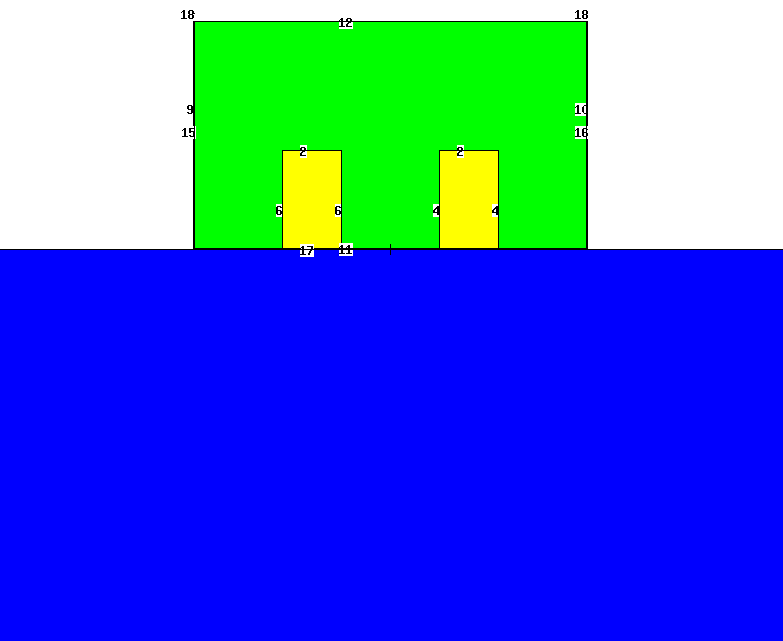
\includegraphics[width=0.3\textwidth]{criticality.png}
      \caption{2D XZ plot of Exercise 3.d. (Graphite) geometry.}
      \label{fig:ex_3_d_2_geometry}
    \end{figure}

\section{Results}
  \subsection{Exercise 1}
    \subsubsection{Initial Simulation}
      \begin{figure}[htb]
        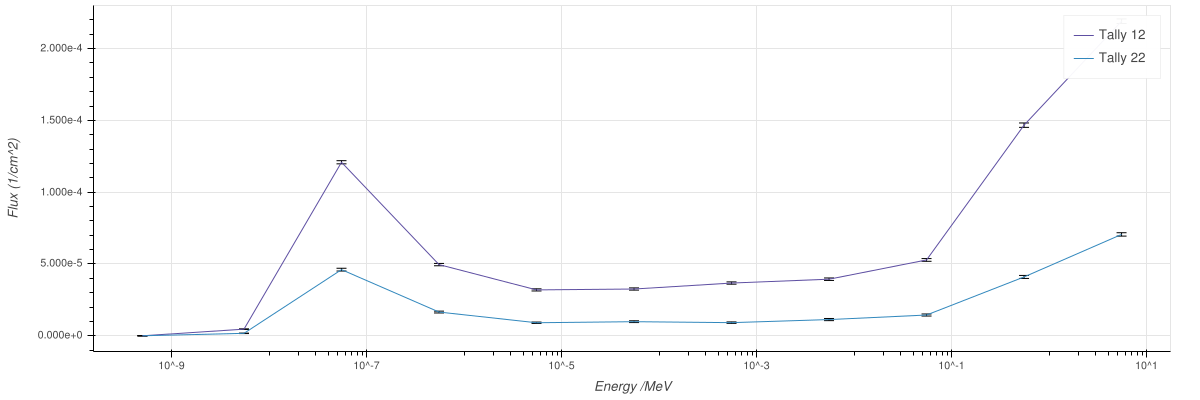
\includegraphics[width=\textwidth]{tallies.png}
        \caption{Fluence tallies for external surfaces of container, for \num{20000} histories. Tally 12 corresponds to the fluence across the shorter sides of the container, 22 the longer sides.}
        \label{fig:tallies_20000}
      \end{figure}

%TODO table
    The tallies are defined as follows:
    \begin{itemize}
      \item Tally 12: The short sides of characteristic length \SI{10}{\cm}
      \item Tally 22: The long sides of characteristic length \SI{20}{\cm}
    \end{itemize}

    For the tallies, MCNP reported that the tallies passed most of the 10 statistical tests for the tally fluctuation chart, which are defined as
    \begin{enumerate}
      \item Mean is randomly distributed
      \item Relative error ideally less than $0.10$
      \item Relative error decreases over time
      \item Decrease rate of relative error follows $\frac{1}{\sqrt{\text{nps}}}$
      \item Variance of variance ideally less than $0.10$
      \item Variance of variance decreases over time
      \item Decrease rate of variance of variance follows $\frac{1}{\sqrt{\text{nps}}}$
      \item Figure of Merit (FoM) is roughly constant
      \item FoM is randomly distributed
      \item Slope of the FoM pdf is greater than $3.0$
    \end{enumerate}
    The first and last tallies passed all ten tests, whilst Tally 22 failed the final FoM slope PDF test. In addition, all tallies had at least one bin with large relative error ($>0.1$).

    The total fluences across each pair of surfaces were as follows
    \begin{itemize}
      \item Long sides (Tally 12): \SI{7.70884\pm0.093277e-4}{\neutron\per\cm^2}
      \item Short sides (Tally 34): \SI{2.53400 \pm 0.082862e-4}{\neutron\per\cm^2}
    \end{itemize}
    \begin{figure}[htb]
      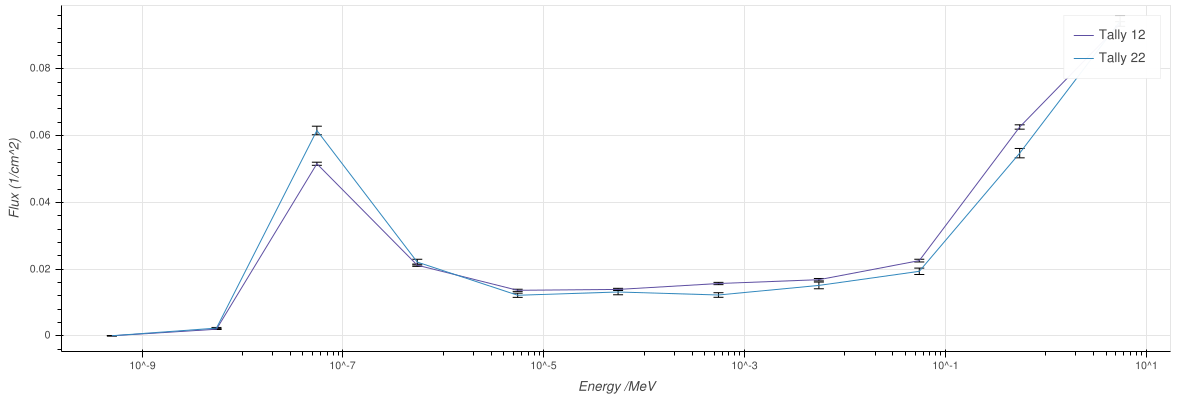
\includegraphics[width=\textwidth]{tallies_norm.png}
      \caption{Area normalised fluence tallies for external surfaces of container, for \num{20000} histories. Tally 12 corresponds to the fluence across the shorter sides of the container, 22 the longer sides.}
      \label{fig:tallies_20000_norm}
    \end{figure}

    \subsubsection{Flux}
    For a source of $10^{10}$ neutrons per second, the corresponding fluxes would be \SI{7.70884\pm 0.093277e+6}{\neutron\per\cm^2\per\second} and \SI{2.53400 \pm 0.082862e+6}{\neutron\per\cm^2\per\second} respectively.

    \subsubsection{Increasing Number of Histories}
      By increasing the particle histories limit to $200000$, the standard uncertainty upon the tally amplitudes diminishes, approximately $\frac{1}{2}$ as expected. The bin amplitude for Tally 22 corresponding to $(\num{1e-8} < x <\num{1e-9})$ did not lie within the uncertainty permitted by its previous value. However, this tally did not pass all statistical tests for $20000$ to allow such a constraint in the first place, and so was to be expected. By increasing the number of particle histories to the new limit, all statistical tests were subsequently passed. Furthermore, the difference in neutron energy distribution between the two tallies became more apparent; in particular, in the higher energy regime the two distributions diverged most significantly, with the narrower surfaces (further from the source) showing greater attenuation at higher energies.
      The recorded fluences were as follows:
      \begin{itemize}
          \item Long sides (Tally 12): \SI{7.65531\pm 0.029856e-4}{\neutron\per\cm^2}
          \item Short sides (Tally 34): \SI{2.5150\pm 0.025402e-4}{\neutron\per\cm^2}
      \end{itemize}

  \subsection{Exercise 3}
    \begin{table}[]
    \centering
    \caption{$k_{\text{eff}}$ for various simulated scenarios.}
    \label{table:reactivities}
    \begin{tabular}{@{}ccc@{}}
    \toprule
    Moderator & Enrichment & $k_{\text{eff}}$
    \\
    \midrule
    Light water        & \SI{20}{\percent} &  \num{0.79340 \pm 0.00075} \\
    Graphite           & \SI{20}{\percent} &  \num{0.93439 \pm 0.00075} \\
    Light water        & \SI{25}{\percent} &  \num{0.84532 \pm 0.00076} \\
    Graphite           & \SI{25}{\percent} &  \num{1.00507 \pm 0.00078} \\
    \bottomrule
    \end{tabular}
    \end{table}


\section{Analysis}
  \subsection{Exercise 1}
    The final FoM slope test evaluates whether the central limit theorem has been satisfied; that is, both the first and second moments of the PDF exist (and are therefore finite). The second moment $\int_{\infty}^{\infty}{x^2f(x)\operatorname{dx}}$ is observed to exist when $f(x)$ decreases faster than $\frac{1}{x^3}$, and hence the final test evaluates this condition. Consequently, in failing this test for the initial simulation, it cannot be concluded that Tally 22 is reliable.

    The significant difference between the total fluences for the two tallies can be explained by both the variation in solid angle between the two surfaces (each surface is sufficiently large relative to the distance to the source, that the incident flux varies along the surface), and the difference in neutron absorption along the axes of the detector. The neutron absorption probability through a medium is given by the Beer Lambert law, and is exponential in the distance travelled.
    The normalised (by area) neutron energy distributions are approximately equal, and what variation there exists between the two tallies lies predominantly within the uncertainty on the recorded values. However, there are several points, particularly in the higher energy regime whose standard errors do not account for the observed deviation. In these cases, the nonlinear attenuation function, which depends upon neutron energy, leads to a distortion of the tallied energy spectrum.

  \subsection{Exercise 3}
    \subsubsection{Graphite Moderator}
    When replacing the moderator material with graphite, the effective criticality of the system was observed to increase. The criticality of a reactor depends upon the number of neutrons which are thermalised (by the moderator) and lead to thermal fission in the fuel. In transitioning the moderator material from light water to graphite, the mean logarithmic energy decrement of the moderator $\xi$ decreases (lesser energy loss per collision), such that the average number of collisions required to thermalise a fast neutron increases by a factor $\frac{\xi_{H_2O}}{\xi_{C}}=5.8\,.$
    However, the scattering to capture ratio of graphite is far higher than that of light water ($1500$ vs $77.17$), and thus its effective "moderating ratio" $\frac{\xi\sigma_{s}}{\sigma_{a}}$ is greater. This result was observed in the predicted $k_{\text{eff}}$ for the two systems. In the case of the graphite moderator,  $k_{\text{eff}}$ was greater (closer to criticality) than that of the light water.
    For both moderators, the application of the Shapiro\textendash Wilke (W) test for normality indicated that the results are normally distributed with a \SI{95}{\percent} confidence interval for all of the reactivity estimators.

    \subsubsection{Increasing Enrichment}
    After increasing the enrichment of the uranium cylinders, the $k_{\text{eff}}$ of both modelled systems was observed to increase. Similarly to the previous configuration, the predicted coefficient for the graphite moderator remained greater than that of the light water.
    As for the previous scenario, the application of the Shapiro\textendash Wilke (W) test for normality indicated that the results are normally distributed with a \SI{95}{\percent} confidence interval for all of the reactivity estimators.

    \begin{figure}
      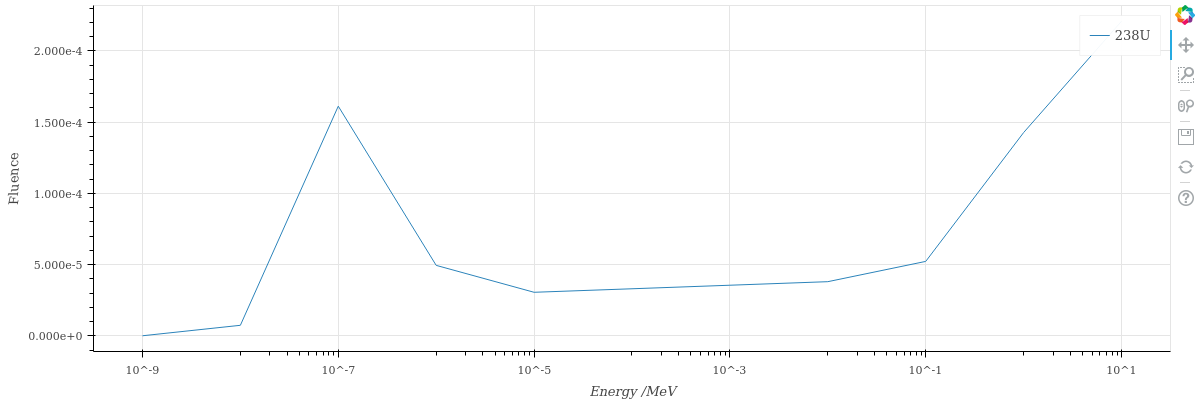
\includegraphics[width=\textwidth]{cross_sections.png}
      \caption{Fission cross sections of \ce{^{238}U} and \ce{^{235}U}}
      \label{fig:cross_sections}
    \end{figure}

    The observed increase in reactivity derives from the increased effective fission cross section of the fuel that follows fuel enrichment (see Fig~\ref{fig:cross_sections}). $^{235}\text{U}$ has a greater fission cross section than $^{238}\text{U}$, and thus increasing the ratio of $^{235}\text{U}$ to $^{238}\text{U}$ in the fuel serves to increase the fission probability, moving the system towards criticality.

\section{Conclusions}
  In completing the two exercises, several important observations were made concerning the various MCNP features which may be used to ensure valid results, and identify problematic cases (such as undersampled paths). The final exercise shows explicitly the importance of selecting the correct fuel enrichment, and moderator material, to avoid a reactor becoming supercritical on prompt neutrons alone.


\section{Appendix}
    \captionof{listing}{Exercise 1. MCNP input file.\label{lst:ex_1}}
    \inputminted[linenos,breaklines]{lexer.py -x}{mcnp/1.ip}

    \captionof{listing}{Exercise 3.d. (Graphite) MCNP input file.\label{lst:ex_3_d_2}}
    \inputminted[linenos,breaklines]{lexer.py -x}{mcnp/3.d.2.ip}
    
\printbibliography

\end{document}
